\documentclass[a4paper,11pt,DIV=12,overfullrule=on]{scrreprt}
\usepackage{unicode-math}
\usepackage{polyglossia}
\setdefaultlanguage{german}
\setotherlanguage{english}
\setmainfont[Mapping=tex-text]{Raleway}
\setmonofont[Mapping=tex-text, Scale=0.9]{Fira Code Light}
\setmathfont{Asana Math}

\usepackage{xltxtra}
\usepackage{microtype}
\usepackage[svgnames, x11names, xetex, rgb, RGB, HTML, hyperref]{xcolor}
\definecolor{shortygreen}{HTML}{0033f2}  % FIXME: Echte Farbwerte eintragen
% \usepackage{listings}
% \lstset{basicstyle=\ttfamily, language=Javascript, numbers=left}
\usepackage[xetex, colorlinks, breaklinks, hyperindex, pdfpagelabels]{hyperref}
\hypersetup{
pdfauthor = {Markus Rennings},
pdftitle = {Shorty – URL-Shortener, Gruppe 3, Projektphase 2},
pdfsubject = {Projektdokumentation Shorty},
pdfkeywords = {Projekt, Projektphase, aws2302, Shorty, URL-Shortener},
pdfcreator = {XeLaTeX with hyperref package},
pdfproducer = {pdfLaTeX},
colorlinks = true,
linkcolor = shortygreen,          % color of internal links
citecolor = green,        % color of links to bibliography
filecolor = magenta,      % color of file links
urlcolor = blue,          % color of external links
}
\usepackage{graphicx}
\graphicspath{ {img/} }%


% Title Page
\subject{Projekt 2, Gruppe 3}
\title{Shorty – URL-Shortener}
\subtitle{}
\author{Andreas Brühl\thanks{Datenbank (Struktur und Anbindung)} \and Deniz Durmaz\thanks{Design, Frontend, Doku} \and Sebastian Hufeld\thanks{Design, Backend} \and Jason Krimmel\thanks{Design, Frontend} \and Markus Rennings\thanks{API-Design, Backend, Infrastruktur, OpenAPI, Doku, \XeLaTeX}}
\date{23.\,August–5.\,September~2023}
\publishers{Betreut durch: Martin Dubb}


\begin{document}
\raggedbottom%
\maketitle

\tableofcontents

% ! 1. Einleitung
\chapter{Einleitung}
\section{Kontext der Arbeit}
Das Projekt wird im Rahmen einer geförderten Weiterbildung erstellt. Der Träger der Weiterbildung ist die \href{https://techstarter.de/}{Techstarter GmbH}. Es gab mehrere Projekte zur Auswahl mit freier Gruppen- und Themenfindung. Das gewählte Projekt ist ein URL Shortener.

\section{Motivation für diese Arbeit}
In der Weiterbildung wurden verschiedene Methoden und Themenbereiche vermittelt. Diese sollen und werden in diesem Full-Stack-Projekt zusammengeführt und genutzt. So soll zum einen gezeigt werden, wie wir diese vielen Teilbereiche nutzen, um das Projekt umzusetzen.

Die größte Problematik ist es, sich erst einmal als Gruppe zu finden, aufzuteilen und zu sortieren, um die Anforderungen umzusetzen.

\section{Zielstellung für diese Arbeit}
Unsere Lösung wandelt lange URLs in kurze und eindeutige URLs um. Bei URLs kann die Zeichenlänge je nach Darstellung in mehreren Zeilen ausarten. Das kann zu Problemen in Dokumenten, Mails oder Social-Media-Post führen. Durch die gekürzten URLs wird dieses Problem behoben oder aber auch, wenn eine Zeichenbegrenzung vorhanden ist, wird diese nicht durch die lange URL kannibalisiert. Optisch sind Short URLs ebenfalls nicht so aufdringlich.

\section{Anforderungen für diese Arbeit}
\begin{description}
    \item[URL-Validierung] Es ist erforderlich, eine URL-Validierung zu implementieren, um sicherzustellen, dass die eingegebenen URLs gültig sind.
    \item[URL-Kürzung] Die Lösung muss in der Lage sein, lange URLs in kurze URLs umzuwandeln.
    \item[Generierung von Kurzlink-Codes] Die Kurzlinks müssen eindeutig sein.
    \item[Benutzeroberfläche] Es muss eine benutzerfreundliche Oberfläche sein, über die Nutzer URLs eingeben und Kurzlinks generieren können.
    \item[Anzeige von Kurzlinks] Eingeloggte Nutzer sollten die Möglichkeit erhalten, bereits erstellte Kurzlinks anzuzeigen (History).
    \item[Datenbank] Die Anwendung muss die ursprünglichen URLs und die zugehörigen Kurzlinks in einer Datenbank speichern und die Verknüpfung zwischen ihnen sicherstellen.
    \item[API] Eine API muss entwickelt werden, um die Interaktion zwischen Frontend und Backend zu ermöglichen. Dies ermöglicht das Erstellen von Kurzlinks und das Abrufen. Das gleiche gilt für die dazugehörigen Statistiken.
    \item[Statistik und Analyse] Die Anwendung muss die Daten über die Nutzung der generierten Kurzlinks sammeln und speichern. Einschließlich Anzahl der Klicks, Zeitpunkt der Nutzung und Informationen zu OS und Browser der Nutzer, müssen generiert werden.
    \item[(Passwortschutz für Link-Bearbeitung und Statistik)] Jeder generierte Kurzlink muss über ein eindeutiges Schlüssel/Passwort verfügen, mit dem Benutzer den Link bearbeiten und die Statistiken einsehen können.
\end{description}

% ! 2. Technische Grundlagen
\chapter{Technische Grundlagen}
\section{Benutzeroberfläche}
\section{Datenbank}
\subsection{Datenbank-Struktur}
\section{Statistik und Analyse}
Für die Statistik nutzen wir die Express.js-Middleware {\ttfamily express-useragent}\footnote{\href{https://www.npmjs.com/package/express-useragent}{https://www.npmjs.com/package/express-useragent}}, welches die User-Agent-Kennung zusammenfasst, so dass man nicht für jede Browser-Version einzeln checken muss. Diese Daten werden in der Datenbank kumuliert und bei Anfrage entsprechend über den API-Endpunkt an den Client gesendet.
%FIXME: Endpunkt? Stats komplett oder aufgeteilt an den Client

\section{API}
\section{URL-Validierung}
Zur Validierung der URL nutzen wir das Paket {\ttfamily url-http}\footnote{\href{https://www.npmjs.com/package/url-http}{https://www.npmjs.com/package/url-http}} mit einer kleinen Wrapper-Funktion, wobei die URL inklusive Schema ({\ttfamily http://} bzw. {\ttfamily https://}) erwartet wird.
\section{URL-Kürzung}
Die eigentliche URL-Kürzung entsteht durch einen Datenbank-Eintrag, der die generierte Kurz-Url (ID) mit der langen URL verknüpft und zusätzlich die statistischen Daten zu jedem Kurzlink speichert.
\subsection{Algorithmus}
Wir haben uns für die Verwendung eines 58-stelligen Alphabets (Base-58) für die Generierung der ID entschieden. Hierzu werden von einem Base62-Alphabet ({\ttfamily[0-9A-Za-z]}) die Zeichen »0« (Null), »I« (Großbuchstabe i), »O« (Großbuchstabe o) und »l« (Kleinbuchstabe L) entfernt, da diese – je nach Schriftart – verwechselt werden können. Hierdurch wird zwar die Anzahl der möglichen IDs eingeschränkt, aber $58^7 =  2\,207\,984\,167\,552$ Möglichkeiten sollten diese immer noch ausreichen.

Die eigentliche Kurz-URL ist dann ein siebenstelliger base58-kodierter String aus einer Kombination aus Teilen des Unix-Zeitstempels (Abb.~\ref{fig:261shorturl} Zeilen 1–3) und einer zweistelligen Zufallszahl (Zeile 4). Zum einfacheren Verbinden beider Zahlen werden diese zunächst als String generiert und erst bei Übergabe an {\ttfamily base58()} als Integer gewandelt (ebenfalls Zeile 4 in Abb.~\ref{fig:261shorturl}).
\begin{figure}%
    \begin{small}%
        \begin{center}%
            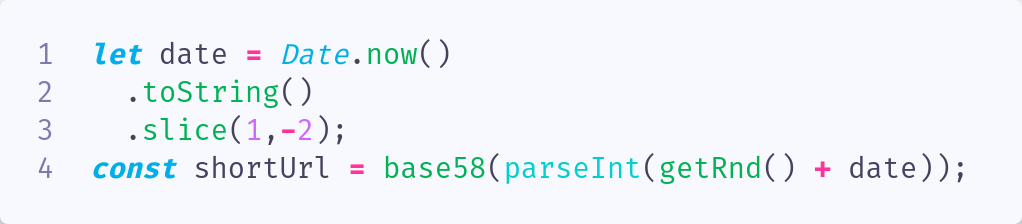
\includegraphics[width=0.8\textwidth]{2_6_1_shortUrl.png}%
        \end{center}%
        \caption{Quelltextauschnitt zur Generierung der Kurz-Url}%
        \label{fig:261shorturl}%
    \end{small}%
\end{figure}%


\section{Passwort für Link-Bearbeitung und Statistik}


% ! 3. Beschreibung der Lösung
\chapter{Beschreibung der Lösung}
\section{Software-Architektur der Lösung}
\section{Übersicht und Zusammenspiel der Komponenten}
\section{Beschreibung der Komponenten}
\subsection{Backend}
\subsubsection{Aufgaben der Komponente}
\subsubsection{Schnittstellen der Komponente}
\subsubsection{Datenstrukturen}
\subsubsection{Funktionsweise}
\subsection{Frontend}
\subsubsection{Sub-Komponente 1}
\paragraph{Aufgabe der Komponente}
\paragraph{Schnittstellen der Komponente}
\subsubsection{Sub-Komponente 2}
\section{Übersicht Verzeichnisse und Dateien}
\section{Bauen des Gesamtsystems}
Ist dies nicht Kapitel 4.1?


% ! 4. Einrichtung und Betrieb der Software-Lösung
\chapter{Einrichtung und Betrieb der Software-Lösung}
\section{Inbetriebnahme der Lösung}
\section{Möglichkeiten zur späteren Anpassung und Weiterentwicklung}

% ! 5. Retrospektive
\chapter{Retrospektive}
\section{Evaluierung der Projektergebnisse}
\section{Bewertung der eigenen Arbeitsweise und die Zusammenarbeit im Team}
\section{Gewonnene Erkenntnisse für zukünftige Projekte}

% ! 6. Zusammenfassung und Ausblick
\chapter{Zusammenfassung und Ausblick}

\listoftables
\listoffigures
\end{document}
